%%%%%%%%%%%%%%%%%%%%%%%%%%%%%%%%%%%%%%%%%
% University/School Laboratory Report
% LaTeX Template
% Version 3.1 (25/3/14)
%
% This template has been downloaded from:
% http://www.LaTeXTemplates.com
%
% Original author:
% Linux and Unix Users Group at Virginia Tech Wiki 
% (https://vtluug.org/wiki/Example_LaTeX_chem_lab_report)
%
% License:
% CC BY-NC-SA 3.0 (http://creativecommons.org/licenses/by-nc-sa/3.0/)
%
%%%%%%%%%%%%%%%%%%%%%%%%%%%%%%%%%%%%%%%%%

%----------------------------------------------------------------------------------------
%	PACKAGES AND DOCUMENT CONFIGURATIONS
%----------------------------------------------------------------------------------------

\documentclass[11pt,a4paper]{article}
\usepackage[utf8]{inputenc}
\usepackage[english,polish]{babel}
%\usepackage[T1]{fontenc}
\usepackage{polski}
\usepackage{amsfonts}
\usepackage[left=3cm,right=3cm,top=3cm,bottom=3cm]{geometry}
\usepackage{siunitx} % Provides the \SI{}{} and \si{} command for typesetting SI units
\usepackage{graphicx} % Required for the inclusion of images
\usepackage{natbib} % Required to change bibliography style to APA
\usepackage{amsmath} % Required for some math elements
\usepackage{epstopdf}
\usepackage[colorlinks=false,urlcolor=blue,citecolor=green]{hyperref}
\usepackage{fancyhdr}
\usepackage{lastpage}
\usepackage{array}
\usepackage{hhline}
\usepackage{svg}
\usepackage{multirow}
\usepackage{enumerate}%[I], numerki, [(a)]
\usepackage{float}

%Figure numbering
\usepackage{chngcntr}
\counterwithin{figure}{section}
\counterwithin{equation}{section}

\newcommand*{\captionsource}[2]{%
  \caption[{#1}]{%
    #1%
    \\\hspace{\linewidth}%
    \textbf{Źródło:} #2%
  }%
}

\AtBeginDocument{
	\renewcommand{\tablename}{Tabela}
	\renewcommand{\figurename}{Rys.}
}

%tabelki
\usepackage{tabularx}
\newcolumntype{A}{>{\centering\arraybackslash}X}
\newcolumntype{B}{>{\centering\arraybackslash} m{0.4\textwidth} }

\setlength\parindent{0pt} % Removes all indentation from paragraphs

\renewcommand{\labelenumi}{\alph{enumi}.} % Make numbering in the enumerate environment by letter rather than number (e.g. section 6)

%\usepackage{times} % Uncomment to use the Times New Roman font

\title{\textbf{Lewitacja magnetyczna}} % Title

\author{Marcin Kowalczyk \\ Maciej Cebula \\ Daniel Rubak} % Author name

\date{26 listopad, 2017} % Date for the report

\begin{document}

\maketitle % Insert the title, author and date

\begin{center}
\begin{tabular}{l r}
Data wykonania: & 21 listopad, 2017 \\ % Date the experiment was performed
Przedmiot: & Laboratorium Problemowe 2 \\
Prowadzący: & Dawid Knapik % Instructor/supervisor
\end{tabular}
\end{center}

\section{Wstęp}
\label{sec:wstep}
Celem projektu było zaprojektowanie systemu sterowania dla układu dwóch rotorów w osiach prostopadłych (model helikoptera). Działanie układu opiera się na generowaniu momentów sił przez obracające się śmigła zamontowane na silnikach prądu stałego. Momenty sił generowane przez grawitację mają być równoważone przez wytworzony moment siły. Moment siły wytwarzany przez silnik jest zależny od współczynnika wypełnienia sygnału PWM podawanego na silnik. Układ umożliwia pomiar orientacji obiektu i prędkości obrotowych silników prądu stałego, sterowanie napięciem podawanym na silniki oraz umożliwia współpracę z urządzeniami sterującymi. Do pomiaru orientacji służą enkodery przyrostowe, natomiast do pomiaru prędkości służą prądnice tachometryczne, w których wytworzone napięcie jest proporcjonalne do mierzonej prędkości obrotowej. Na początku postanowiono wykonać układ sterowania dla helikoptera z zablokowaną osią pionową.

Do symulacji, obliczeń numerycznych i generowania kodu wykorzystano programy \textit{Matlab} i \textit{Simulink}. Wygenerowany kod jest wykonywany w czasie rzeczywistym. Możliwa jest również zmiana parametrów układu sterowania (np. pozycji zadanej) w czasie pracy układu. Mierzone wielkości są również wyświetlane na bieżąco w programie \textit{Simulink}.

\section{Model matematyczny}
\label{sec:modelmatematyczny}
Wykorzystano następujący model matematyczny układu dla osi poziomej:
\begin{equation}
\begin{aligned}
J_v \frac{d^2\alpha_v}{dt^2} &= -f_v\frac{d\alpha_v}{dt}+a\cdot sin(\alpha_v-\alpha_{v0})+M_v(\omega_v)\\
I_v\frac{d\omega_v}{dt} &= u_v - H_v^{-1}(\omega_v)
\end{aligned}
\label{eq:model_vertical}
\end{equation}
\noindent gdzie:\newline
\(\alpha_v\) jest kątem obrotu w płaszczyźnie pionowej,\newline
\(J_v\) jest momentem bezwładności względem osi obrotu w płaszczyźnie pionowej,\newline
\(f_v\) jest współczynnikiem tarcia lepkiego,\newline
\(a\) jest momentem sił grawitacji,\newline
\(\alpha_{v0}\) jest kątem równowagi układu w płaszczyźnie pionowej,\newline
\(I_v\) jest momentem bezwładności dużego śmigła,\newline
\(H_v^{-1}(\omega_v)\) jest charakterystyką statyczną układu silnik-śmigło dla silnika głównego,\newline
\(\omega_v\) jest prędkością obrotową silnika głównego,\newline
\(M_v(\omega_v)\) jest momentem sił generowanym przez silnik główny,\newline
\(u_v\) jest współczynnikiem wypełniania sygnału PWM dla silnika głównego.
\paragraph*{}
Dla osi pionowej wykorzystano następujący model matematyczny układu:
\begin{equation}
\begin{aligned}
J_h \frac{d^2\alpha_h}{dt^2} &= -f_h\frac{d\alpha_h}{dt}+M_h(\omega_h)\\
I_h\frac{d\omega_h}{dt} &= u_h - H_h^{-1}(\omega_h)
\end{aligned}
\label{eq:model_horizontal}
\end{equation}
\noindent gdzie:\newline
\(\alpha_h\) jest kątem obrotu w płaszczyźnie poziomej,\newline
\(J_h\) jest momentem bezwładności względem osi obrotu w płaszczyźnie poziomej,\newline
\(f_h\) jest współczynnikiem tarcia lepkiego,\newline
\(I_h\) jest momentem bezwładności małego śmigła,\newline
\(H_h^{-1}(\omega_h)\) jest charakterystyką statyczną układu silnik-śmigło dla silnika bocznego,\newline
\(\omega_h\) jest prędkością obrotową silnika bocznego,\newline
\(M_h(\omega_h)\) jest momentem sił generowanym przez silnik boczny,\newline
\(u_h\) jest współczynnikiem wypełniania sygnału PWM dla silnika bocznego.
\paragraph*{}
Przyjęto, że wielkości \(M_v(\omega_v)\), \(M_h(\omega_h)\), \(H_v^{-1}(\omega_v)\) i \(H_h^{-1}(\omega_h)\) są wielomianami piątego stopnia. Równania różniczkowe \eqref{eq:model_vertical} i \eqref{eq:model_horizontal} są więc równaniami nieliniowymi.

Równania \eqref{eq:model_vertical} i \eqref{eq:model_horizontal} przekształcono do postaci równań stanu. Dla równań \eqref{eq:model_vertical} mają one następującą postać:
\begin{equation}
\begin{aligned}
\dot x_1 &= x_2\\
\dot x_2 &= -\frac{f_v}{J_v}x_2+\frac{a}{J_v}\sin (\alpha_v-\alpha_{v0})+\frac{M_v(\omega_v)}{J_v}\\
\dot x_3 &= \frac{u_v}{I_v}-\frac{H_v^{-1}(\omega_v)}{I_v}
\end{aligned}
\end{equation}

Natomiast dla równań \eqref{eq:model_horizontal} mają następującą postać:
\begin{equation}
\begin{aligned}
\dot x_1 &= x_2\\
\dot x_2 &= -\frac{f_h}{J_h}x_2+\frac{M_h(\omega_h)}{J_h}\\
\dot x_3 &= \frac{u_h}{I_h}-\frac{H_h^{-1}(\omega_h)}{I_h}
\end{aligned}
\end{equation}

\section{Identyfikacja}
\label{sec:identyfikacja}
Zagadnienie identyfikacji modeli nieliniowych jest bardzo często zagadnieniem problematycznym. Dla modeli liniowych wystarczy zazwyczaj wykorzystać metodę najmniejszych kwadratów. Dla modelu nieliniowego metoda ta daje na ogół obciążoną estymację parametrów, a rozwiązanie zadania może być niejednoznaczne. Oprócz tego zadanie to jest skomplikowane pod względem numerycznym, gdyż rozwiązywania nieliniowych równań różniczkowych jest złożone obliczeniowo. Aby ułatwić identyfikację należy zdekomponować ją na znacznie prostsze zadania. Dzięki temu identyfikacja modelu nieliniowego sprowadza się do wykonania kilkudziesięciu pomiarów oraz odpowiednich przekształceń algebraicznych.

\subsection{Prędkość kątowa z prądnicy tachometrycznej}
W pierwszej kolejności konieczne było przeliczenie napięcia z prądnicy tachometrycznej na prędkość kątową w radianach na sekundę. W tym celu wykorzystano dostępną dokumentację oraz zmierzone dane. Dla danej wartości współczynnika wypełnienia PWM odczytywano multimetrem napięcie na wyprowadzeniach z prądnicy tachometrycznej oraz wartość wyświetlaną w \textit{Simulink}. W dokumentacji sprawdzono jak należy przeliczyć napięcie prądnicy tachometrycznej na prędkość kątową. Punkty pomiarowe następnie aproksymowano wielomianem pierwszego stopnia. Wyniki zostały zaprezentowane na rysunku \ref{fig:char_V_U}.

\begin{figure}[h]
	\centering
	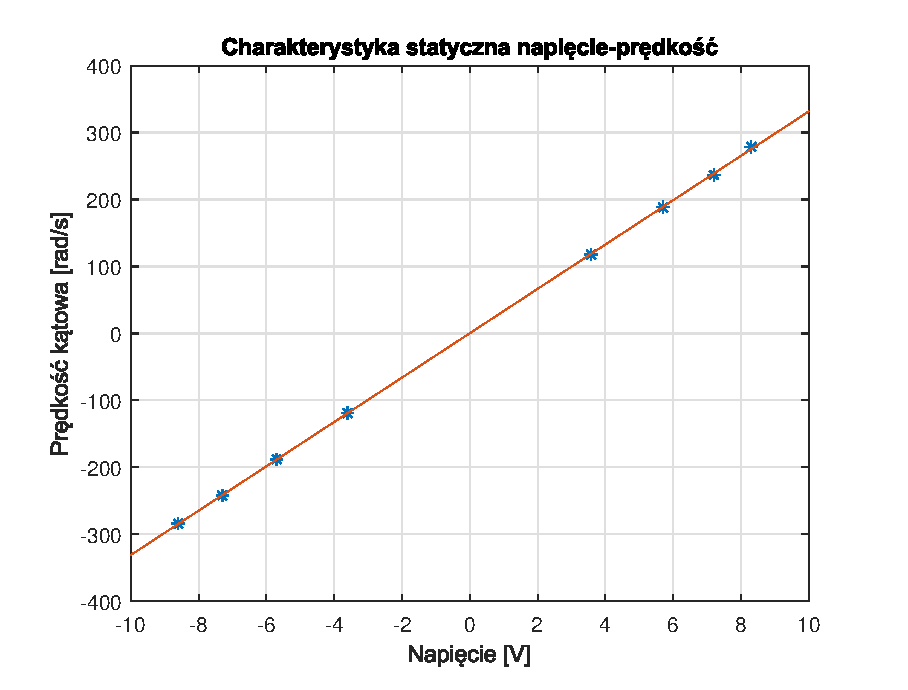
\includegraphics[width=4in]{Figures/char_V_U.eps}
	\caption{Charakterystyka statyczna prędkości kątowej od odczytu z czujnika.}
	\label{fig:char_V_U}
\end{figure}

Otrzymano wzór \eqref{eq:V_Vs} opisujący przeliczenie wielkości odczytanej w \textit{Simulink} na prędkość kątową w radianach na sekundę.
\begin{equation}
V = \frac{2000\pi}{0.52\cdot 60}(0.1644V_S+0.0019)
\label{eq:V_Vs}
\end{equation}
\noindent gdzie:\newline
\(V_S\) jest wartością odczytaną w \textit{Simulink},\newline
\(V\) jest prędkością kątową w radianach na sekundę.

\subsection{Moment niewyważenia}
Wykonano badanie momentu niewyważenia, który powodował,że kiedy na układ nie działały żadne dodatkowe siły, to nie znajdował się on w pozycji poziomej. Rozpoczęto od zgrubnego wyznaczenia kąta równowagi w płaszczyźnie pionowej. W tym celu użyto elektronicznej "poziomicy" w postaci telefonu komórkowego. Wyznaczony kąt miał wartość:
\begin{equation}
\alpha_{v0} = -0.491
\end{equation}
Następnie wykorzystano równanie \eqref{eq:moment_niewywazenia} do wyznaczenia zależności momentu niewyważenia od kąta nachylenia (parametru \(a\)).
\begin{equation}
J_v \frac{d^2\alpha_v}{dt^2} = -f_v\frac{d\alpha_v}{dt}+a\cdot \sin(\alpha_v-\alpha_{v0})+M_v(\omega_v)
\label{eq:moment_niewywazenia}
\end{equation}
W pewnej odległości \(l\) od osi obrotu przyłożono siłę (pochodzącą od zawieszonych ciężarków), której moment był przeciwny do momentu niewyważenia. Wagę ciężarków dobrano tak, by powstały moment równoważył niewyważenie dla kąta \(\alpha_v=0\). Kąt ten nie zmienia się, a więc jego pochodne są równe \(0\). Można więc zapisać równania \eqref{eq:M_zew} opisujące równowagę sił w tej sytuacji.
\begin{equation}
\begin{aligned}
M_{zew} &= -a\cdot \sin(\alpha_v-\alpha_{v0})\\
M_{zew} &= lmg\cos(\alpha_v)
\end{aligned}
\label{eq:M_zew}
\end{equation}
\noindent gdzie:\newline
\(a\) jest maksymalnym momentem sił niewyważenia,\newline
\(\alpha_v\) jest kątem obrotu w płaszczyźnie pionowej,\newline
\(\alpha_{v0}\) jest kątem równowagi układu w płaszczyźnie pionowej,\newline
\(M_{zew}\) jest przyłożonym momentem sił,\newline
\(l\) jest odległością od osi obrotu do punktu przyłożenia zewnętrznej siły,\newline
\(m\) jest łączną masą przyłożonych ciężarków,\newline
\(g\) jest przyspieszeniem ziemskim.
\paragraph*{}
Opisane parametry miały następujące wartości:
\begin{equation}
\begin{aligned}
\alpha_v &= 0\\
\alpha_{v0} &= -0.491\\
l &= 0.26\si{m}\\
m &= 0.06\si{kg}\\
g &= 9.81\si{m/s^2}
\end{aligned}
\end{equation}
Podstawiając wartości powyższych parametrów do wzorów \eqref{eq:M_zew} wyznaczono następującą wartość współczynnika momentu niewyważenia:
\begin{equation}
a = -0.3068\si{Nm}
\end{equation}

\subsection{Moment siły generowany przez silnik główny}
Następnie konieczne było wyznaczenie momentu siły generowanego przez śmigło przymocowane do silnika głównego. W tym celu podawano różne wartości współczynnika wypełnienia PWM na silnik. Po ustaleniu się prędkości obrotowej zawieszano ciężarki w pewnej odległości od osi obrotu tak, aby przyłożony zewnętrzny moment siły równoważył moment siły wygenerowany przez silnik oraz moment niewyważenia dla kąta \(\alpha_v=0\). W tym celu ponownie wykorzystano równanie \eqref{eq:moment_niewywazenia}. Kąt nachylenia nie zmieniał się, a więc pochodne kąta nachylenia po czasie wynosiły \(0\). Wzór ten sprowadzał się więc do zależności opisanej wzorem
\begin{equation}
\begin{aligned}
M_v(\omega_v) &= -a\cdot \sin(\alpha_v-\alpha_{v0})-M_{zew}\\
M_{zew} &= lmg\cos(\alpha_v)
\end{aligned}
\label{eq:moment_sily_glowny}
\end{equation}
\noindent gdzie:\newline
\(a\) jest maksymalnym momentem sił niewyważenia,\newline
\(\alpha_v\) jest kątem obrotu w płaszczyźnie pionowej,\newline
\(\alpha_{v0}\) jest kątem równowagi układu w płaszczyźnie pionowej,\newline
\(M_{zew}\) jest przyłożonym momentem sił,\newline
\(M_v(\omega_v)\) jest momentem siły generowanym przez silnik główny,\newline
\(\omega_v\) jest prędkością obrotową silnika głównego,\newline
\(l\) jest odległością od osi obrotu do punktu przyłożenia zewnętrznej siły,\newline
\(m\) jest łączną masą przyłożonych ciężarków,\newline
\(g\) jest przyspieszeniem ziemskim.
\paragraph*{}
Zależność momentu siły nośnej od prędkości kątowej postanowiono aproksymować wielomianem piątego stopnia. Na wykresie \ref{fig:char_M_V} kolorem czerwonym zaznaczone zostały wyznaczone punkty pomiarowe, natomiast kolorem niebieskim funkcja aproksymująca (wielomian).

\begin{figure}[h]
	\centering
	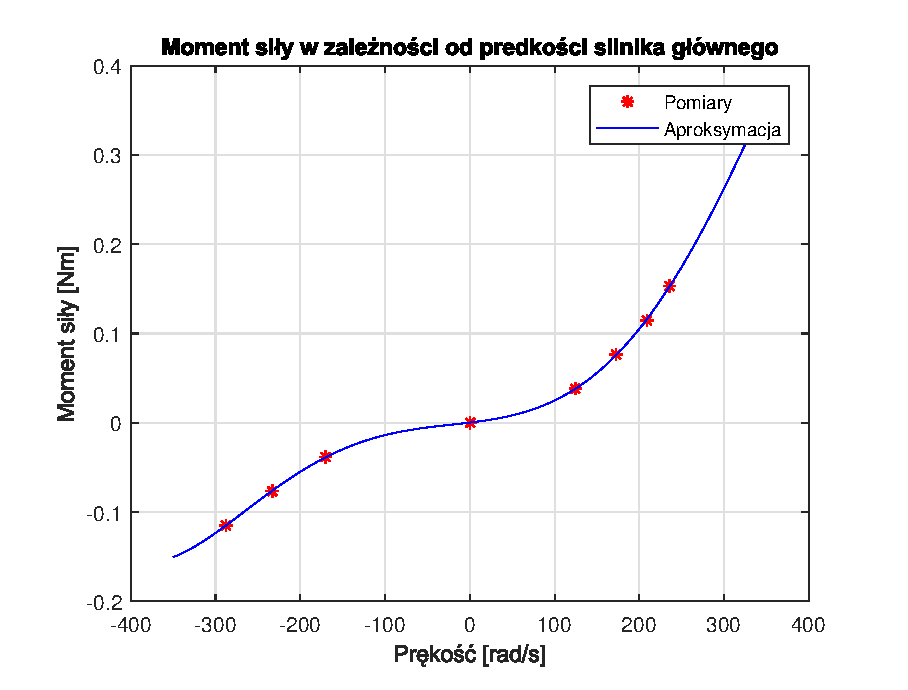
\includegraphics[width=4in]{Figures/char_M_V.eps}
	\caption{Charakterystyka statyczna momentu siły nośnej od prędkości obrotowej silnika.}
	\label{fig:char_M_V}
\end{figure}

Badana zależność wyraża się następującym wzorem:
\begin{equation}
\begin{aligned}
M_v(\omega_v) &= -2.5146\cdot 10^{-14}\omega_v^5+2.9593\cdot 10^{-12}\omega_v^4+8.1312\cdot 10^{-9}\omega_v^3\\ & \quad +5.0407\cdot 10^{-7}\omega_v^2+1.1510\cdot 10^{-4}\omega_v+2.7833\cdot 10^{-4}
\end{aligned}
\end{equation}

\subsection{Zależność oporów ruchu od prędkości obrotowej śmigła głównego}
Kolejnym krokiem procesu identyfikacji było badanie wpływu prędkości obrotowej silnika na napięcie podawane na silnik. Większa prędkość obrotowa powoduje większe opory, przez co mniejsze napięcie podawane jest na silnik. Opisuje to równanie \eqref{eq:domega_v}.
\begin{equation}
I_v\frac{d\omega_v}{dt} = u_v - H_v^{-1}(\omega_v)
\label{eq:domega_v}
\end{equation}
\noindent gdzie:\newline
\(I_v\) jest momentem bezwładności dużego śmigła,\newline
\(H_v^{-1}(\omega_v)\) jest charakterystyką statyczną układu silnik-śmigło dla silnika głównego,\newline
\(\omega_v\) jest prędkością obrotową silnika głównego,\newline
\(u_v\) jest współczynnikiem wypełniania sygnału PWM dla silnika głównego.
\paragraph*{}
Pomiary wykonywane są dla ustalonej prędkości obrotowej silnika, więc jej pochodne po czasie są równe \(0\). Stąd powyższe równie przyjmuje następującą postać:
\begin{equation}
H_v^{-1}(\omega_v) = u_v
\end{equation}
Zależność oporów ruchu śmigła od prędkości kątowej postanowiono aproksymować wielomianem piątego stopnia. Na wykresie \ref{fig:char_U_V} kolorem czerwonym zaznaczone zostały wyznaczone punkty pomiarowe, natomiast kolorem niebieskim funkcja aproksymująca (wielomian).

\begin{figure}[h]
	\centering
	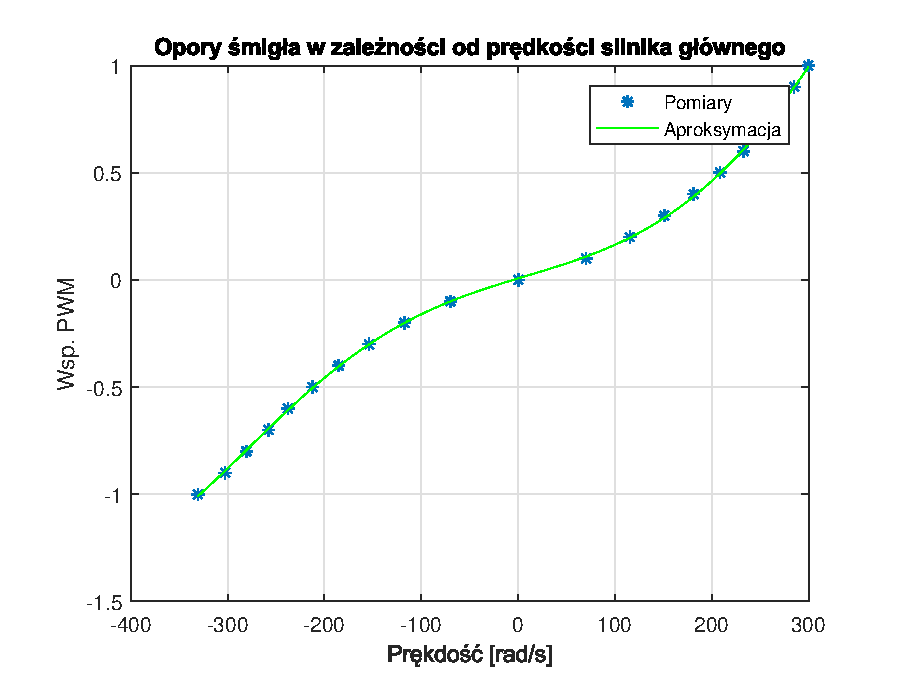
\includegraphics[width=4in]{Figures/char_U_V.eps}
	\caption{Charakterystyka statyczna oporów ruchu śmigła od prędkości obrotowej silnika.}
	\label{fig:char_U_V}
\end{figure}

Badana zależność wyraża się następującym wzorem:
\begin{equation}
\begin{aligned}
H_v^{-1}(\omega_v) &= -7.4418\cdot 10^{-14}\omega_v^5+1.3631\cdot 10^{-11}\omega_v^4+2.6232\cdot 10^{-8}\omega_v^3\\ & \quad -6.6054\cdot 10^{-7}\omega_v^2+0.0014\omega_v+0.0072
\end{aligned}
\end{equation}

\subsection{Parametry modelu układu silnik DC - śmigło główne}
Następnie przeprowadzono identyfikację parametrów równania \eqref{eq:uklad_silnik_smiglo_v}.
\begin{equation}
I_v\frac{d\omega_v}{dt} = u_v - H_v^{-1}(\omega_v)
\label{eq:uklad_silnik_smiglo_v}
\end{equation}
Funkcja \(H_v^{-1}(\omega_v)\) została już zidentyfikowana. Należy więc dobrać tylko wartość momentu bezwładności dużego śmigła (\(I_v\)). W tym celu zarejestrowano odpowiedź prędkości obrotowej śmigła na skok wartości współczynnika wypełniania sygnału PWM podawanego na silnik. Następnie z wykorzystaniem funkcji \textit{lsqnonlin} programu \textit{MATLAB} znaleziono taką wartość tego parametru, która minimalizuje błąd średniokwadratowy odpowiedzi modelu względem zarejestrowanego przebiegu. Do rozwiązywania równania różniczkowego \eqref{eq:uklad_silnik_smiglo_v} w procesie optymalizacji użyto funkcji \textit{ode45}. Na rysunku \ref{fig:ident_I_v} kolorem niebieskim przedstawiono zarejestrowany przebieg, a kolorem czerwonym odpowiedź aproksymowanego modelu.

\begin{figure}[H]
	\centering
	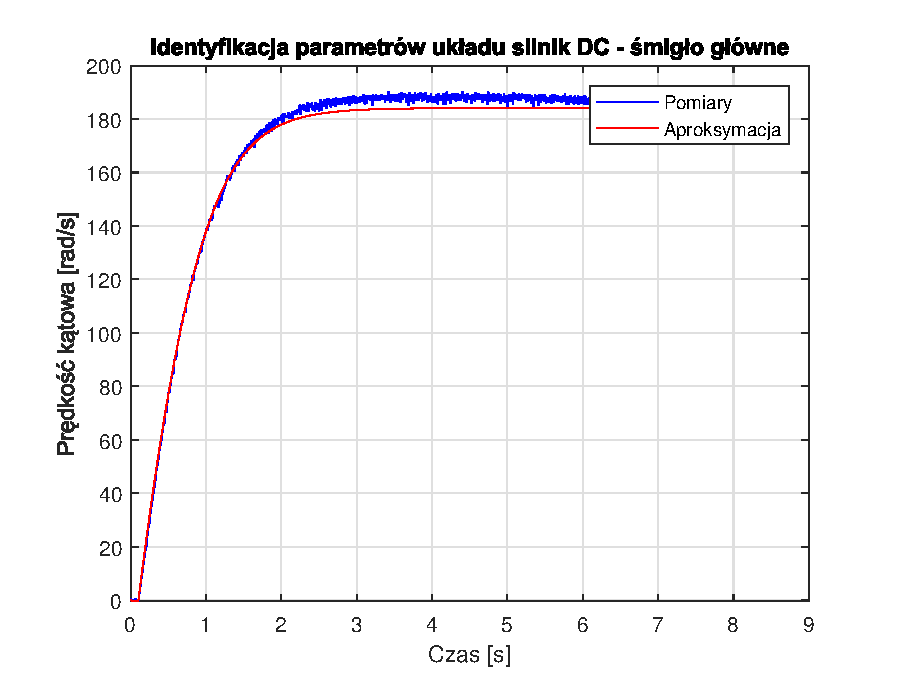
\includegraphics[width=4in]{Figures/ident_I_v.eps}
	\caption{Porównanie odpowiedzi zarejestrowanej i aproksymowanego modelu.}
	\label{fig:ident_I_v}
\end{figure}

Wyznaczony parametr miał następującą wartość:
\begin{equation}
I_v = 0.0017\si{kg.m^2}
\end{equation}

\subsection{Moment bezwładności kładu dla osi poziomej}
Ostatnimi koniecznymi do zbadania parametrami dla układu w płaszczyźnie pionowej były jego moment bezwładności, współczynnik tarcia lepkiego oraz dokładna wartość kąta równowagi układu. Wielkości te zostały wyznaczone na podstawie równania \eqref{eq:ident_J_v}.
\begin{equation}
J_v \frac{d^2\alpha_v}{dt^2} = -f_v\frac{d\alpha_v}{dt}+a\cdot sin(\alpha_v-\alpha_{v0})+M_v(\omega_v)
\label{eq:ident_J_v}
\end{equation}
Identyfikację tej części przeprowadzano wprowadzając układ w drgania wokół punktu równowagi. W trakcie eksperymentu silnik był wyłączony. Równanie \eqref{eq:ident_J_v} sprowadza się więc do postaci:
\begin{equation}
J_v \frac{d^2\alpha_v}{dt^2} = -f_v\frac{d\alpha_v}{dt}+a\cdot sin(\alpha_v-\alpha_{v0})
\end{equation}
Zapisano przebieg kąta wychylenia układu podczas eksperymentu. Następnie szukano parametrów \(J_v\), \(f_v\) oraz \(alpha_{v0}\) takich, by minimalizowały średniokwadratowy wskaźnik jakości. Wykorzystano do tego funkcję \textit{lsqnonlin} programu \textit{MATLAB}. Na rysunku \ref{fig:ident_J_v} kolorem niebieskim przedstawiono zarejestrowany przebieg, a kolorem czerwonym odpowiedź aproksymowanego modelu.

\begin{figure}[H]
	\centering
	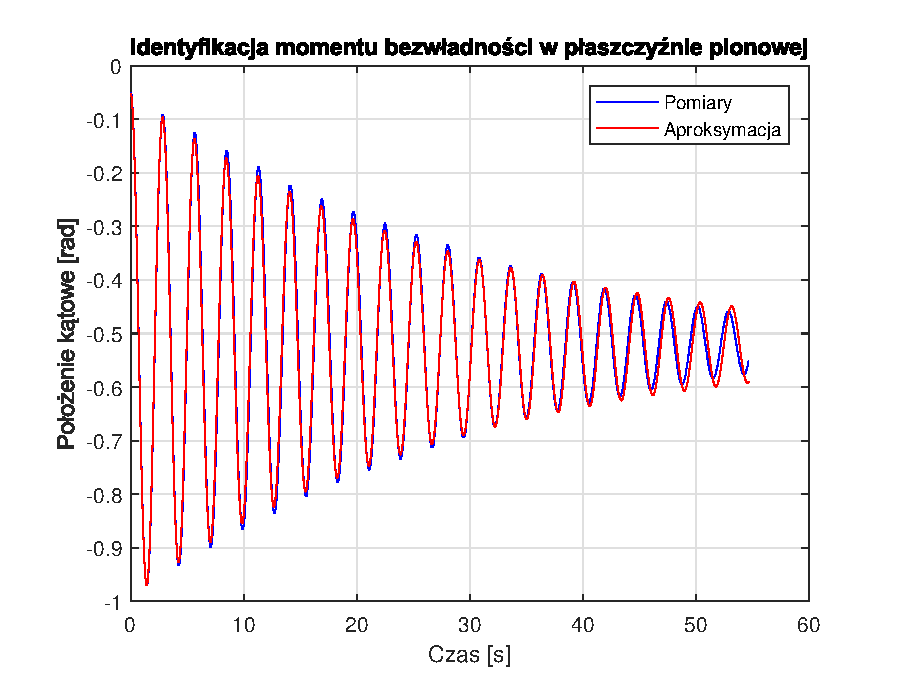
\includegraphics[width=4in]{Figures/ident_J_v.eps}
	\caption{Porównanie odpowiedzi zarejestrowanej i aproksymowanego modelu.}
	\label{fig:ident_J_v}
\end{figure}

W wyniku optymalizacji otrzymano następujące wartości poszukiwanych parametrów modelu:
\begin{equation}
\begin{aligned}
J_v &= 0.0604\si{kg.m^2}\\
f_v &= 0.0042\si{Nm.s}\\
\alpha_{v0} &= -0.5223
\end{aligned}
\end{equation}

\subsection{Zależność oporów ruchu od prędkości obrotowej śmigła bocznego}
Następnie zbadano wpływ prędkości obrotowej silnika na napięcie podawane na silnik dl osi pionowej. Podobnie jak dla osi poziomej, większa prędkość obrotowa powoduje większe opory, przez co mniejsze napięcie pod awane jest na silnik. Opisuje to równanie \eqref{eq:domega_h}.
\begin{equation}
I_h\frac{d\omega_h}{dt} = u_h - H_h^{-1}(\omega_h)
\label{eq:domega_h}
\end{equation}
\noindent gdzie:\newline
\(I_h\) jest momentem bezwładności śmigła bocznego,\newline
\(H_h^{-1}(\omega_h)\) jest charakterystyką statyczną układu silnik-śmigło dla silnika bocznego,\newline
\(\omega_h\) jest prędkością obrotową silnika bocznego,\newline
\(u_h\) jest współczynnikiem wypełniania sygnału PWM dla silnika bocznego.
\paragraph*{}
Pomiary wykonano są dla ustalonej prędkości obrotowej silnika, więc jej pochodne po czasie są równe \(0\). Stąd powyższe \eqref{eq:domega_h} przyjmuje następującą postać:
\begin{equation}
H_h^{-1}(\omega_h) = u_h
\end{equation}
Zależność oporów ruchu śmigła od prędkości kątowej postanowiono aproksymować wielomianem piątego stopnia. Na wykresie \ref{fig:char_U_V_az} kolorem czerwonym zaznaczone zostały wyznaczone punkty pomiarowe, natomiast kolorem niebieskim funkcja aproksymująca (wielomian).

\begin{figure}[H]
	\centering
	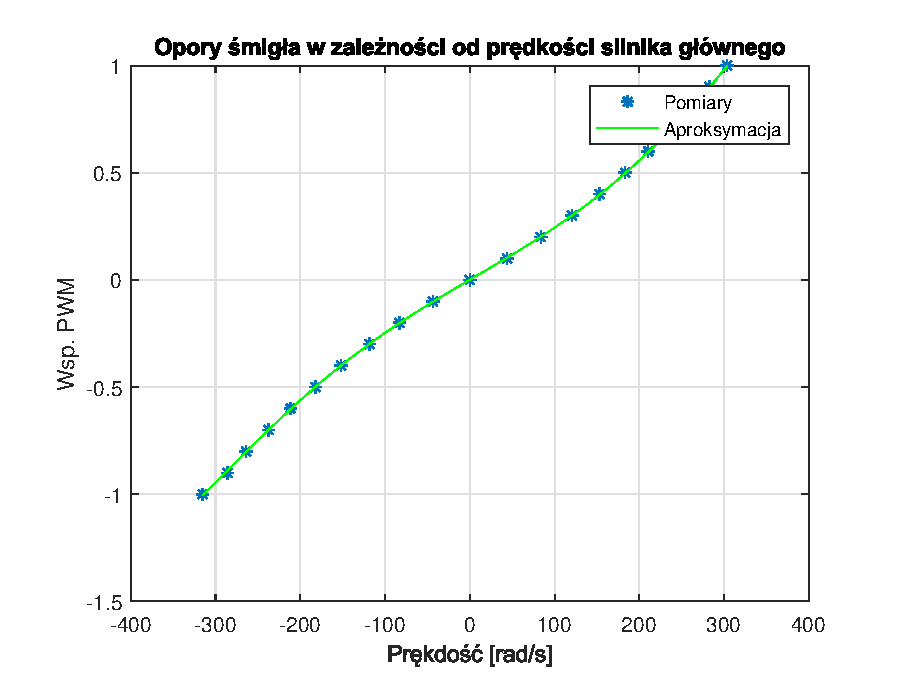
\includegraphics[width=4in]{Figures/char_U_V_az.eps}
	\caption{Charakterystyka statyczna oporów ruchu śmigła bocznego od prędkości obrotowej silnika.}
	\label{fig:char_U_V_az}
\end{figure}

Badana zależność wyraża się następującym wzorem:
\begin{equation}
\begin{aligned}
H_h^{-1}(\omega_h) &= -4.0004\cdot 10^{-14}\omega_h^5+5.1822\cdot 10^{-12}\omega_h^4+1.3426\cdot 10^{-8}\omega_h^3\\ & \quad -2.8251\cdot 10^{-7}\omega_h^2+0.0023\omega_h+6.8066\cdot 10^{-4}
\end{aligned}
\end{equation}

\subsection{Parametry modelu układu silnik DC - śmigło boczne}
Konieczne było przeprowadzenie identyfikacji parametrów równania \eqref{eq:uklad_silnik_smiglo_h}.
\begin{equation}
I_h\frac{d\omega_h}{dt} = u_h - H_h^{-1}(\omega_h)
\label{eq:uklad_silnik_smiglo_h}
\end{equation}
Funkcja \(H_h^{-1}(\omega_h)\) została zidentyfikowana w poprzednim podrozdziale. Należy więc dobrać wartość momentu bezwładności śmigła bocznego (\(I_h\)). W tym celu zarejestrowano odpowiedź prędkości obrotowej śmigła na skok wartości współczynnika wypełniania sygnału PWM podawanego na silnik. Następnie dla zarejestrowanego przebiegu użyto funkcję \textit{lsqnonlin} programu \textit{MATLAB}, by znaleźć taką wartość parametru \(I_h\), która minimalizuje błąd średniokwadratowy odpowiedzi modelu. Do rozwiązywania równania różniczkowego \eqref{eq:uklad_silnik_smiglo_h} w procesie optymalizacji użyto funkcji \textit{ode45}. Na rysunku \ref{fig:ident_I_h} kolorem niebieskim przedstawiono zarejestrowany przebieg, a kolorem czerwonym odpowiedź aproksymowanego modelu.

\begin{figure}[H]
	\centering
	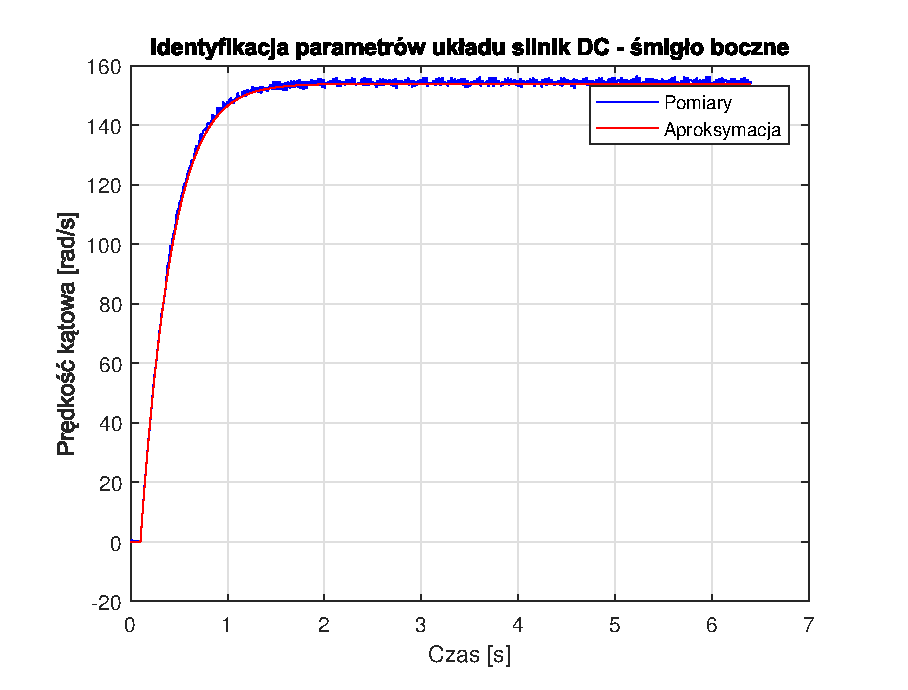
\includegraphics[width=4in]{Figures/ident_I_h.eps}
	\caption{Porównanie zapisanego przebiegu i odpowiedzi zidentyfikowanego modelu.}
	\label{fig:ident_I_h}
\end{figure}

Wyznaczony parametr miał następującą wartość:
\begin{equation}
I_h = 8.7148\cdot 10^{-4}\si{kg.m^2}
\end{equation}

\subsection{Moment siły generowany przez silnik boczny}
Przeprowadzono również eksperyment w celu wyznaczenia momentu siły generowanego przez śmigło boczne. W tym celu podawano różne wartości współczynnika wypełnienia PWM na silnik przy zablokowanym układzie. Po ustaleniu się prędkości obrotowej układ uwalniano i zapisywano przebiegi położenia kątowego i prędkości obrotowej silnika. W tym celu wykorzystano równanie \eqref{eq:moment_sily_boczny}.
\begin{equation}
J_h \frac{d^2\alpha_h}{dt^2} = -f_h\frac{d\alpha_h}{dt}+M_h(\omega_h)
\label{eq:moment_sily_boczny}
\end{equation}
\noindent gdzie:\newline
\(\alpha_h\) jest kątem obrotu w płaszczyźnie poziomej,\newline
\(J_h\) jest momentem bezwładności względem osi obrotu w płaszczyźnie poziomej,\newline
\(f_h\) jest współczynnikiem tarcia lepkiego,\newline
\(\omega_h\) jest prędkością obrotową silnika bocznego,\newline
\(M_h(\omega_h)\) jest momentem sił generowanym przez silnik boczny.
\paragraph*{}
W celu zmniejszenia ilości parametrów koniecznych do optymalizacji postanowiono obie strony równania podzielić przez \(J_h\). Otrzymane równanie poddano procesowi identyfikacji.Na wykresie \ref{fig:V_ident_J_h} przedstawiono prędkość obrotową silnika. Jest ona w przybliżeniu stała (pomijając szumy pomiarowe). Można więc założyć, że również moment wywołany tą prędkością jest stały. W związku z tym identyfikacja sprowadza się do znalezienia parametru \(f_v\) i stałego momentu siły.

\begin{figure}[H]
	\centering
	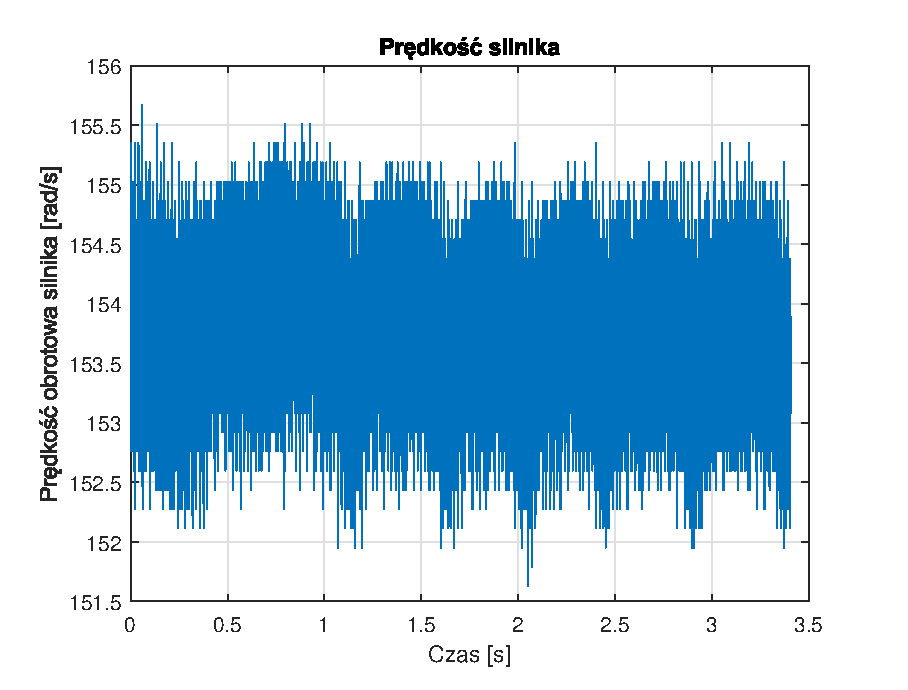
\includegraphics[width=4in]{Figures/V_ident_J_h.eps}
	\caption{Prędkość obrotowa silnika w trakcie eksperymentu.}
	\label{fig:V_ident_J_h}
\end{figure}

Dla zarejestrowanych przebiegów użyto funkcji \textit{lsqnonlin} programu \textit{MATLAB}, by znaleźć takie wartości współczynników, które minimalizują błąd średniokwadratowy odpowiedzi modelu. Do rozwiązywania równania różniczkowego \eqref{eq:moment_sily_boczny} w procesie optymalizacji użyto funkcji \textit{ode45}. Na rysunku \ref{fig:ident_J_h} kolorem niebieskim przedstawiono jeden z zarejestrowanych przebiegów, a kolorem czerwonym odpowiedź aproksymowanego modelu.

\begin{figure}[H]
	\centering
	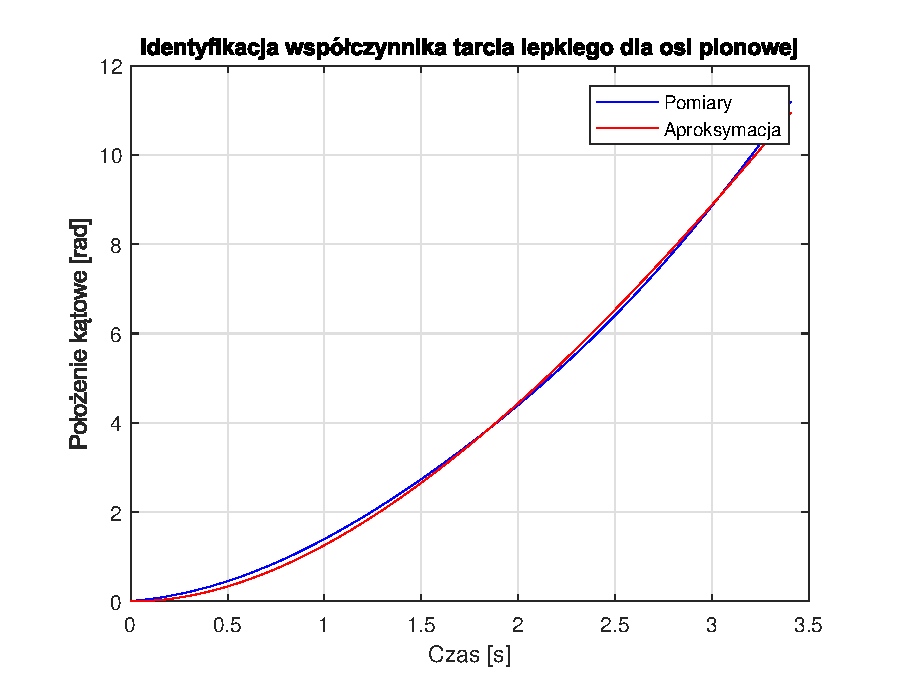
\includegraphics[width=4in]{Figures/ident_J_h.eps}
	\caption{Porównanie zarejestrowanej odpowiedzi z aproksymowanym modelem.}
	\label{fig:ident_J_h}
\end{figure}

Wyznaczony parametr \(f_h\) miał następującą wartość:
\begin{equation}
f_h = 0.0539
\end{equation}
Następnie zarejestrowano dane z eksperymentów, podczas których układ nie był zablokowany po podaniu skoku współczynnika wypełnienia sygnału PWM na silnik. Dane te znacznie lepiej nadają się do zidentyfikowania współczynników wielomianu \(M_h(\omega_h)\). Na wykresie \ref{fig:V_ident_M_h} przedstawiono przebieg prędkości obrotowej silnika podczas jednego z przeprowadzonych eksperymentów.

\begin{figure}[H]
	\centering
	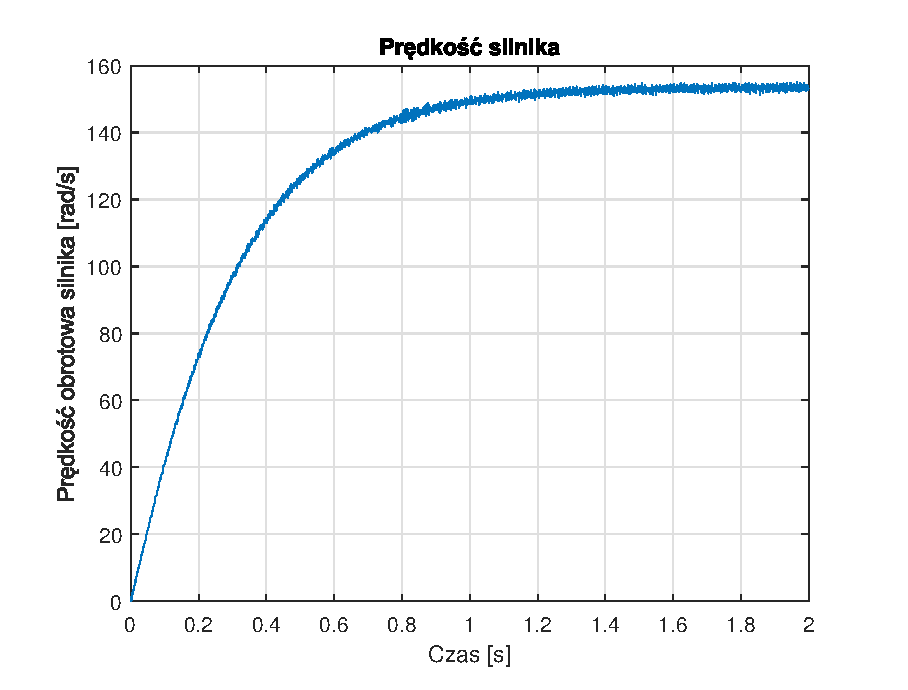
\includegraphics[width=4in]{Figures/V_ident_M_h.eps}
	\caption{Prędkość obrotowa silnika w trakcie eksperymentu.}
	\label{fig:V_ident_M_h}
\end{figure}

Za pomocą funkcji \textit{lsqnonlin} wyznaczono współczynniki wielomianu \(M_h(\omega_h)\), które minimalizowały średniokwadratowy wskaźnik jakości dla zarejestrowanych przebiegów. Na wykresach \ref{fig:ident_M_h_04} i \ref{fig:ident_M_h_-06} kolorem niebieskim oznaczono zarejestrowany przebieg, a kolorem czerwonym odpowiedź aproksymowanego modelu. Pierwszy z wykresów odpowiada skokowi współczynnika wypełnienia do wartości 0.4, natomiast drugi skokowi tej wielkości do -0.6 (silnik obracający się w przeciwną stronę).

\begin{figure}[H]
	\centering
	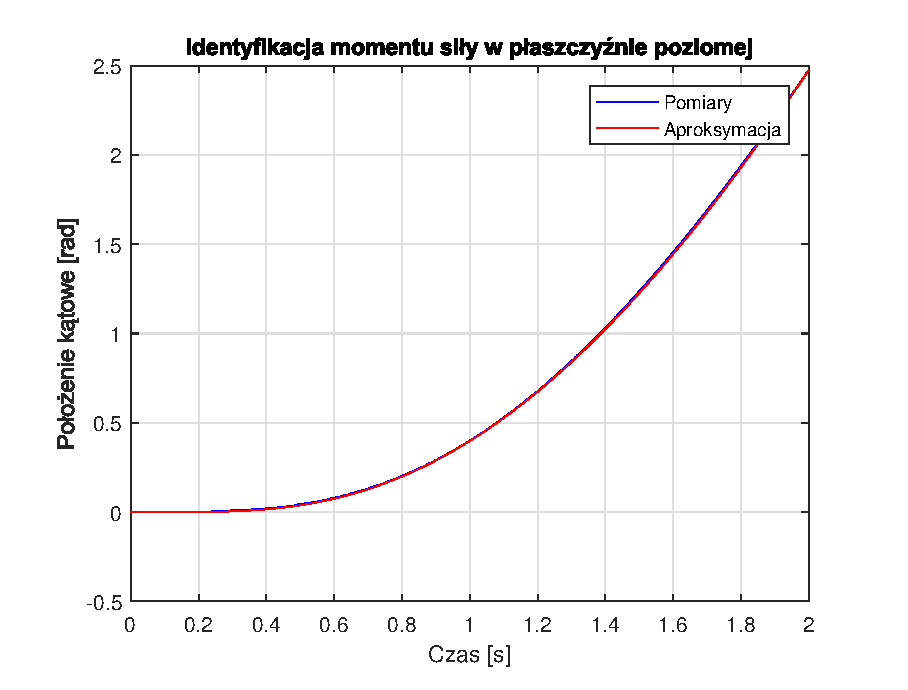
\includegraphics[width=4in]{Figures/ident_M_h_04.eps}
	\caption{Porównanie odpowiedzi dla współczynnika wypełnienia PWM równego \(0.4\).}
	\label{fig:ident_M_h_04}
\end{figure}

\begin{figure}[H]
	\centering
	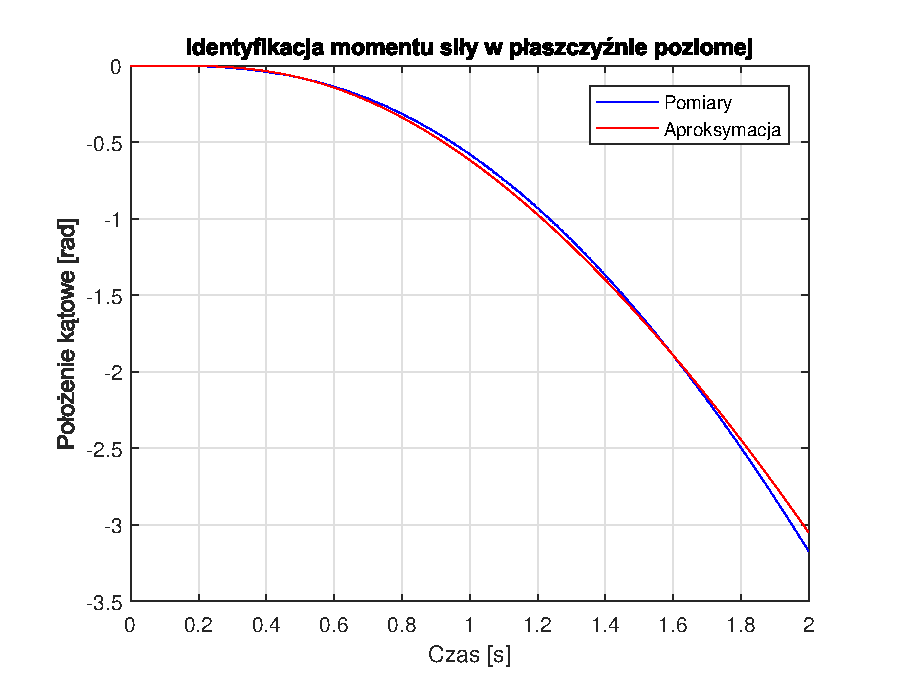
\includegraphics[width=4in]{Figures/ident_M_h_-06.eps}
	\caption{Porównanie odpowiedzi dla współczynnika wypełnienia PWM równego \(-0.6\).}
	\label{fig:ident_M_h_-06}
\end{figure}

Na rysunku \ref{fig:ident_M_h} przedstawiono wykres wyznaczonej funkcji momentu siły zależnej od prędkości obrotowej silnika bocznego \(M_h(\omega_h)\).

\begin{figure}[H]
	\centering
	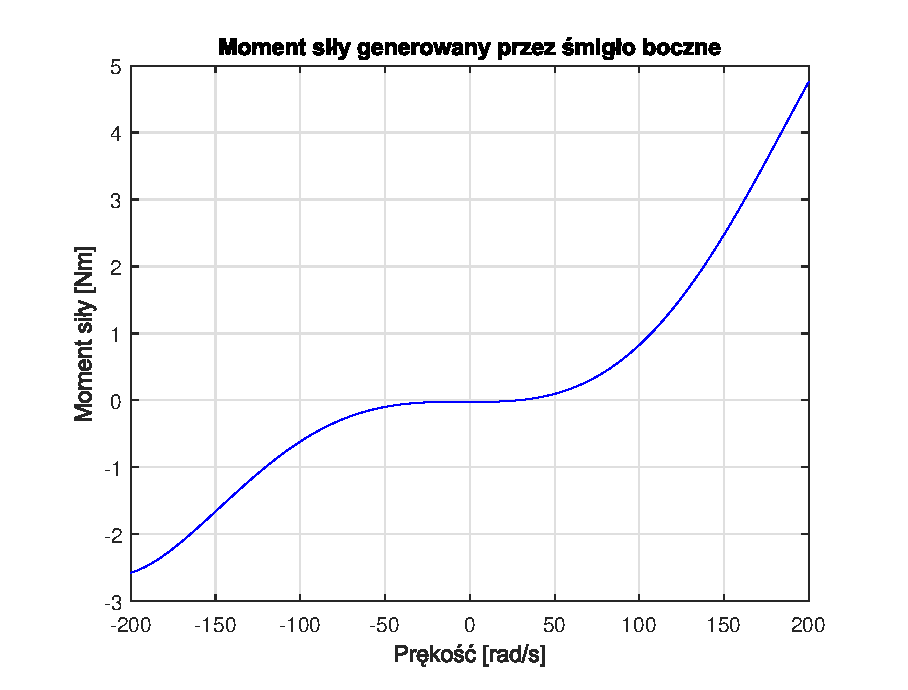
\includegraphics[width=4in]{Figures/ident_M_h.eps}
	\caption{Moment siły w zależności od prędkości obrotowej silnika bocznego.}
	\label{fig:ident_M_h}
\end{figure}

Powyższa funkcja opisana jest następującym wzorem:
\begin{equation}
\begin{aligned}
M_h(\omega_h) &= -8.8567\cdot 10^{-12}\omega_h^5+4.9851\cdot 10^{-10}\omega_h^4+8.1331\cdot 10^{-7}\omega_h^3\\ & \quad +7.9455\cdot 10^{-6}\omega_h^2-3.3890\cdot 10^{-5}\omega_h-0.0215
\end{aligned}
\end{equation}

\section{Punkt równowagi}
\label{sec:punktrownowagi}
W dalszej części pracy projektowano sterowanie układem z zablokowanym ruchem w płaszczyźnie poziomej. W tym celu konieczne było wyznaczenie zbioru punktów równowagi systemu. Punkt spełnia następujące równania:
\begin{equation}
\begin{aligned}
\dot x_1 &= 0\\
\dot x_2 &= 0\\
\dot x_3 &= 0
\end{aligned}
\end{equation}
A więc:
\begin{equation}
\begin{aligned}
0 &= x_2\\
0 &= -\frac{f_v}{J_v}x_2+\frac{a}{J_v}\sin (\alpha_v-\alpha_{v0})+\frac{M_v(\omega_v)}{J_v}\\
0 &= \frac{u_v}{I_v}-\frac{H_v^{-1}(\omega_v)}{I_v}
\end{aligned}
\label{punkt_rownowagi}
\end{equation}

%\section{Model zlinearyzowany}
%\label{sec:modelzlinearyzowany}
%Do przeprowadzenia dalszych prac niezbędny był zlinearyzowany model układu w otoczeniu punktu pracy. Jest to model liniowy, który w otoczeniu punktu równowagi zachowuje się tak samo lub podobnie do modelu nieliniowego. W tym celu konieczne było najpierw wyznaczenie zbioru punktów równowagi układu. Po kilku przekształceniach otrzymano następujący wynik:
%\begin{equation}
%\begin{aligned}
%x_1&\in[0, 0.02]\\
%x_2&=0\\
%x_3&=\sqrt{\frac{bmg}{a}e^{\frac{x_1}{b}}}\\
%u&=\frac{x_3-u_c}{k}
%\end{aligned}
%\label{eq:equilibrium}
%\end{equation}
%Po podstawieniu zidentyfikowanych parametrów otrzymuje się następujące równania:
%\begin{equation}
%\begin{aligned}
%x_1&\in[0, 0.02]\\
%x_2&=0\\
%x_3&=\sqrt{0.2115e^{\frac{x_1}{0.0067}}}\\
%u&=\frac{x_3}{2.8964}
%\end{aligned}
%\end{equation}
%
%Aby znaleźć macierze A,B,C należy wyliczyć pochodne prawych stron układu równań \eqref{eq:ss}.
%Wyliczone macierze mają następującą postać:
%\begin{equation}
%\begin{aligned}
%A&=\begin{bmatrix}
%0 & 1 & 0\\
%\frac{a}{b^2m}x_3^2e^{-\frac{x_1}{b}} & 0 & \frac{2}{m}x_3\frac{dL(x_1)}{dx_1}\\
%\frac{ku+u_c-x_3}{f(x_1)^2}\frac{df(x_1)}{dx_1} & 0 & -\frac{1}{f(x_1)}
%\end{bmatrix}\\
%B&=\begin{bmatrix}
%0\\
%0\\
%\frac{k}{f(x_1)}
%\end{bmatrix}\\
%C&=\begin{bmatrix}
%1 & 0 & 0\\
%0 & 1 & 0\\
%0 & 0 & 1
%\end{bmatrix}\\
%f(x_1)&=\frac{a}{b}e^{-\frac{x_1}{b}}
%\end{aligned}
%\end{equation}
%Układ został zlinearyzowany w punkcie, dla którego sfera znajduje się w odległości 10 mm od cewki. Dla tego punktu otrzymano następujące macierze układu liniowego:
%\begin{equation}
%\begin{aligned}
%A&=\begin{bmatrix}
%0 & 1 & 0\\
%693.903 & 0 & -9.615\\
%0 & 0 & -863.948
%\end{bmatrix}\\
%B&=\begin{bmatrix}
%0\\
%0\\
%2502.3
%\end{bmatrix}\\
%C&=\begin{bmatrix}
%1 & 0 & 0\\
%0 & 1 & 0\\
%0 & 0 & 1
%\end{bmatrix}
%\end{aligned}
%\label{eq:linearized}
%\end{equation}
%
%Zaimplementowano obliczanie punktu równowagi w modelu \textit{Simulink}. Wielkości te są potrzebne w zadaniu stabilizacji w określonym punkcie. Konieczne jest wtedy obliczenie sterowania w danym punkcie. Schemat realizujący te obliczenia przedstawiony jest na rysunku \ref{eq:equilibrium}.
%
%\begin{figure}[H]
%	\centering
%	\includegraphics[width=2in]{Figures/equilibrium.png}
%	\caption{Schemat \textit{Simulink} realizujący obliczenie punktu równowagi.}
%	\label{fig:equilibrium}
%\end{figure}
%
%\section{Regulator LQ}
%\label{sec:regulatorlq}
%Dla układu zlinearyzowanego opisanego równaniem \eqref{eq:linearized} obliczono macierz wzmocnień regulatora LQ. Regulator ten minimalizuje następujący wskaźnik jakości:
%\begin{equation}
%\begin{aligned}
%J&=\int\limits_0^{\infty}(x^TQx+u^TRu)dt\\
%Q&=\begin{bmatrix}
%1 & 0 & 0\\
%0 & 1 & 0\\
%0 & 0 & 1
%\end{bmatrix}\\
%R&=1
%\end{aligned}
%\end{equation}
%Potrzebne obliczenia (rozwiązanie algebraicznego równania Riccatiego) zostały wykonane za pomocą funkcji programu \textit{Matlab} - \textit{lqr}. Otrzymana macierz wzmocnień ma następującą postać:
%\begin{equation}
%K=\begin{bmatrix}
%-154.245 & -5.940 & 0.734
%\end{bmatrix}
%\end{equation}
%Regulator ten został następnie zaimplementowany w programie \textit{Simulink}. Układ z tym regulatorem został przedstawiony na rysunku \ref{fig:lewitacja_lq}.
%
%\begin{figure}[H]
%	\centering
%	\includegraphics[width=5.5in]{Figures/Lewitacja_LQ.eps}
%	\caption{Układ sterowania lewitacją magnetyczną z regulatorem LQ.}
%	\label{fig:lewitacja_lq}
%\end{figure}
%
%Najpierw przetestowano zadanie stabilizacji modelu układu w odległości 10 mm. Zostało one przedstawione na wykresach od \ref{fig:model_LQ_x1} do \ref{fig:model_LQ_u}.
%
%\begin{figure}[H]
%	\centering
%	\includegraphics[width=4.5in]{Figures/model_LQ_x1.eps}
%	\caption{Zadanie stabilizacji modelu z regulatorem LQ - położenie sfery.}
%	\label{fig:model_LQ_x1}
%\end{figure}
%
%\begin{figure}[H]
%	\centering
%	\includegraphics[width=4.5in]{Figures/model_LQ_x2.eps}
%	\caption{Zadanie stabilizacji modelu z regulatorem LQ - prędkość sfery.}
%	\label{fig:model_LQ_x2}
%\end{figure}
%
%\begin{figure}[H]
%	\centering
%	\includegraphics[width=4.5in]{Figures/model_LQ_x3.eps}
%	\caption{Zadanie stabilizacji modelu z regulatorem LQ - prąd cewki.}
%	\label{fig:model_LQ_x3}
%\end{figure}
%
%\begin{figure}[H]
%	\centering
%	\includegraphics[width=4.5in]{Figures/model_LQ_u.eps}
%	\caption{Zadanie stabilizacji modelu z regulatorem LQ - sterowanie.}
%	\label{fig:model_LQ_u}
%\end{figure}
%
%Regulator LQ stabilizował model, lecz można zauważyć duży uchyb ustalony. Następnie przeprowadzono doświadczenie na rzeczywistym układzie. Pierwszym zadaniem również była stabilizacja układu w odległości 10 mm. Zostało one przedstawione na wykresach od \ref{fig:LQ_stab_pos} do \ref{fig:LQ_stab_con}.
%
%\begin{figure}[H]
%	\centering
%	\includegraphics[width=4.5in]{Figures/LQ_stab_pos.eps}
%	\caption{Zadanie stabilizacji układu z regulatorem LQ - położenie sfery.}
%	\label{fig:LQ_stab_pos}
%\end{figure}
%
%\begin{figure}[H]
%	\centering
%	\includegraphics[width=4.5in]{Figures/LQ_stab_vel.eps}
%	\caption{Zadanie stabilizacji układu z regulatorem LQ - prędkość sfery.}
%	\label{fig:LQ_stab_vel}
%\end{figure}
%
%\begin{figure}[H]
%	\centering
%	\includegraphics[width=4.5in]{Figures/LQ_stab_cur.eps}
%	\caption{Zadanie stabilizacji układu z regulatorem LQ - prąd cewki.}
%	\label{fig:LQ_stab_cur}
%\end{figure}
%
%\begin{figure}[H]
%	\centering
%	\includegraphics[width=4.5in]{Figures/LQ_stab_con.eps}
%	\caption{Zadanie stabilizacji układu z regulatorem LQ - sterowanie.}
%	\label{fig:LQ_stab_con}
%\end{figure}
%
%Następnie przetestowano odpowiedź skokową układu. W tym celu poczekano na ustabilizowanie pozycji sfery, a następnie skokowo zmieniono wartość zadaną. Wykresy od \ref{fig:LQ_step_pos} do \ref{fig:LQ_step_con} przedstawiają zarejestrowaną odpowiedź skokową.
%
%\begin{figure}[H]
%	\centering
%	\includegraphics[width=4.5in]{Figures/LQ_step_pos.eps}
%	\caption{Odpowiedź skokowa układu z regulatorem LQ - położenie sfery.}
%	\label{fig:LQ_step_pos}
%\end{figure}
%
%\begin{figure}[H]
%	\centering
%	\includegraphics[width=4.5in]{Figures/LQ_step_vel.eps}
%	\caption{Odpowiedź skokowa układu z regulatorem LQ - prędkość sfery.}
%	\label{fig:LQ_step_vel}
%\end{figure}
%
%\begin{figure}[H]
%	\centering
%	\includegraphics[width=4.5in]{Figures/LQ_step_cur.eps}
%	\caption{Odpowiedź skokowa układu z regulatorem LQ - prąd cewki.}
%	\label{fig:LQ_step_cur}
%\end{figure}
%
%\begin{figure}[H]
%	\centering
%	\includegraphics[width=4.5in]{Figures/LQ_step_con.eps}
%	\caption{Odpowiedź skokowa układu z regulatorem LQ - sterowanie.}
%	\label{fig:LQ_step_con}
%\end{figure}
%
%Wykresy \ref{fig:LQ_stab_pos} i \ref{fig:LQ_step_pos} potwierdzają to, co zauważono w odpowiedziach modelu dla regulatora LQ. Przy zastosowaniu tego regulatora występuje duży uchyb ustalony. Porównując odpowiedzi modelu i rzeczywistego układu można również wnioskować, że w układzie występują znacznie większe zakłócenia, niż dodane w modelu. Postanowiono również zbadać działanie regulatora LQ dla zadania nadążania. W tym wypadku jako pozycję zadaną podawano funkcję \(0.01+0.002\sin(2\pi t)\), gdzie t oznacza czas. Zadanie nadążania zostało przedstawione na wykresach od \ref{fig:LQ_sin_pos} do \ref{fig:LQ_sin_con}.
%
%\begin{figure}[H]
%	\centering
%	\includegraphics[width=4.5in]{Figures/LQ_sin_pos.eps}
%	\caption{Zadanie nadążania układu z regulatorem LQ - położenie sfery.}
%	\label{fig:LQ_sin_pos}
%\end{figure}
%
%\begin{figure}[H]
%	\centering
%	\includegraphics[width=4.5in]{Figures/LQ_sin_vel.eps}
%	\caption{Zadanie nadążania układu z regulatorem LQ - prędkość sfery.}
%	\label{fig:LQ_sin_vel}
%\end{figure}
%
%\begin{figure}[H]
%	\centering
%	\includegraphics[width=4.5in]{Figures/LQ_sin_cur.eps}
%	\caption{Zadanie nadążania układu z regulatorem LQ - prąd cewki.}
%	\label{fig:LQ_sin_cur}
%\end{figure}
%
%\begin{figure}[H]
%	\centering
%	\includegraphics[width=4.5in]{Figures/LQ_sin_con.eps}
%	\caption{Zadanie nadążania układu z regulatorem LQ - sterowanie.}
%	\label{fig:LQ_sin_con}
%\end{figure}
%
%Na podstawie powyższych wykresów można zaobserwować, że amplituda położenia sfery jest większa niż amplituda pozycji zadanej. Oprócz tego są one względem siebie przesunięte w fazie. Zauważalne jest również zniekształcenie sinusoidy spowodowane nieliniowością systemu lewitacji magnetycznej.
%
%\section{Regulator LQI}
%\label{sec:regulatorlqi}
%Aby pozbyć się uchybu ustalonego postanowiono użyć regulatora LQI. Jest to regulator LQ dla którego w modelu obiektu został wprowadzony dodatkowy, sztuczny stan, który jest proporcjonalny do całki z uchybu. Nowy wektor stanu ma więc następującą postać:
%\begin{equation}
%x=\begin{bmatrix}
%x_1\\
%x_2\\
%x_3\\
%x_4
%\end{bmatrix}
%\end{equation}
%\noindent Gdzie:\newline
%\(x_1\) jest położeniem sfery.\newline
%\(x_2\) jest prędkością sfery.\newline
%\(x_3\) jest prądem cewki.\newline
%\(x_4\) jest całką z uchybu.\newline
%\paragraph*{}
%Macierze zlinearyzowanych równań stanu dla regulatora LQI mają więc następującą postać:
%\begin{equation}
%\begin{aligned}
%A&=\begin{bmatrix}
%0 & 1 & 0 & 0\\
%693.903 & 0 & -9.615 & 0\\
%0 & 0 & -863.948 & 0\\
%1 & 0 & 0 & 0
%\end{bmatrix}\\
%B&=\begin{bmatrix}
%0\\
%0\\
%2502.3\\
%0
%\end{bmatrix}\\
%C&=\begin{bmatrix}
%1 & 0 & 0 & 0\\
%0 & 1 & 0 & 0\\
%0 & 0 & 1 & 0\\
%0 & 0 & 0 & 1
%\end{bmatrix}
%\end{aligned}
%\end{equation}
%
%Macierz wzmocnień dla regulatora LQI wyznaczono ponownie z użyciem funkcji programu \textit{Matlab} - \textit{lqr}. Regulator LQI ma minimalizować następującą funkcję kosztu:
%\begin{equation}
%\begin{aligned}
%J&=\int\limits_0^{\infty}(x^TQx+u^TRu)dt\\
%Q&=\begin{bmatrix}
%1 & 0 & 0 & 0\\
%0 & 1 & 0 & 0\\
%0 & 0 & 1 & 0\\
%0 & 0 & 0 & 1
%\end{bmatrix}\\
%R&=1
%\end{aligned}
%\end{equation}
%Wyznaczona została następująca macierz wzmocnień dla regulatora LQI:
%\begin{equation}
%K=\begin{bmatrix}
%-162.271 & -4.3266 & 0.8074 & -1.0000
%\end{bmatrix}
%\end{equation}
%Regulator ten został również zaimplementowany w programie \textit{Simulink}. Układ z tym regulatorem został przedstawiony na rysunku \ref{fig:lewitacja_slx}.
%
%\begin{figure}[H]
%	\centering
%	\includegraphics[width=5.5in]{Figures/Lewitacja_slx.eps}
%	\caption{Układ sterowania lewitacją magnetyczną z regulatorem LQI.}
%	\label{fig:lewitacja_slx}
%\end{figure}
%
%Na schemacie \ref{fig:lewitacja_slx} widoczna jest metoda obliczania zmiennej \(x_4\). Jest ona obliczana poprzez całkowanie zmiennej \(x_1\). Na podstawie wykonanych doświadczeń postanowiono również zwiększyć wzmocnienie regulatora dla zmiennej \(x_4\), aby przyspieszyć wygasanie oscylacji położenia wokół pozycji zadanej. Najpierw przetestowano zadanie stabilizacji modelu układu w odległości 10 mm. Zostało one przedstawione na wykresach od \ref{fig:model_LQI_x1} do \ref{fig:model_LQI_u}.
%
%\begin{figure}[H]
%	\centering
%	\includegraphics[width=4.5in]{Figures/model_LQI_x1.eps}
%	\caption{Zadanie stabilizacji modelu z regulatorem LQI - położenie sfery.}
%	\label{fig:model_LQI_x1}
%\end{figure}
%
%\begin{figure}[H]
%	\centering
%	\includegraphics[width=4.5in]{Figures/model_LQI_x2.eps}
%	\caption{Zadanie stabilizacji modelu z regulatorem LQI - prędkość sfery.}
%	\label{fig:model_LQI_x2}
%\end{figure}
%
%\begin{figure}[H]
%	\centering
%	\includegraphics[width=4.5in]{Figures/model_LQI_x3.eps}
%	\caption{Zadanie stabilizacji modelu z regulatorem LQI - prąd cewki.}
%	\label{fig:model_LQI_x3}
%\end{figure}
%
%\begin{figure}[H]
%	\centering
%	\includegraphics[width=4.5in]{Figures/model_LQI_u.eps}
%	\caption{Zadanie stabilizacji modelu z regulatorem LQI - sterowanie.}
%	\label{fig:model_LQI_u}
%\end{figure}
%
%Regulator LQI również stabilizował model i w tym wypadku nie ma uchybu ustalonego. Następnie przeprowadzono doświadczenie na rzeczywistym układzie. Pierwszym zadaniem również była stabilizacja układu w odległości 10 mm. Zostało one przedstawione na wykresach od \ref{fig:LQI_stab_pos} do \ref{fig:LQI_stab_con}.
%
%\begin{figure}[H]
%	\centering
%	\includegraphics[width=4.5in]{Figures/LQI_stab_pos.eps}
%	\caption{Zadanie stabilizacji układu z regulatorem LQI - położenie sfery.}
%	\label{fig:LQI_stab_pos}
%\end{figure}
%
%\begin{figure}[H]
%	\centering
%	\includegraphics[width=4.5in]{Figures/LQI_stab_vel.eps}
%	\caption{Zadanie stabilizacji układu z regulatorem LQI - prędkość sfery.}
%	\label{fig:LQI_stab_vel}
%\end{figure}
%
%\begin{figure}[H]
%	\centering
%	\includegraphics[width=4.5in]{Figures/LQI_stab_cur.eps}
%	\caption{Zadanie stabilizacji układu z regulatorem LQI - prąd cewki.}
%	\label{fig:LQI_stab_cur}
%\end{figure}
%
%\begin{figure}[H]
%	\centering
%	\includegraphics[width=4.5in]{Figures/LQI_stab_con.eps}
%	\caption{Zadanie stabilizacji układu z regulatorem LQI - sterowanie.}
%	\label{fig:LQI_stab_con}
%\end{figure}
%
%Powyższe wykresy potwierdzają wnioski z modelu. Regulator LQI poprawnie stabilizuje pozycję i pozwala na usunięcie uchybu ustalonego. Następnie przetestowano odpowiedź skokową układu. W tym celu poczekano na ustabilizowanie pozycji sfery, a następnie skokowo zmieniono wartość zadaną. Wykresy od \ref{fig:LQI_step_pos} do \ref{fig:LQI_step_con} przedstawiają zarejestrowaną odpowiedź skokową.
%
%\begin{figure}[H]
%	\centering
%	\includegraphics[width=4.5in]{Figures/LQI_step_pos.eps}
%	\caption{Odpowiedź skokowa układu z regulatorem LQI - położenie sfery.}
%	\label{fig:LQI_step_pos}
%\end{figure}
%
%\begin{figure}[H]
%	\centering
%	\includegraphics[width=4.5in]{Figures/LQI_step_vel.eps}
%	\caption{Odpowiedź skokowa układu z regulatorem LQI - prędkość sfery.}
%	\label{fig:LQI_step_vel}
%\end{figure}
%
%\begin{figure}[H]
%	\centering
%	\includegraphics[width=4.5in]{Figures/LQI_step_cur.eps}
%	\caption{Odpowiedź skokowa układu z regulatorem LQI - prąd cewki.}
%	\label{fig:LQI_step_cur}
%\end{figure}
%
%\begin{figure}[H]
%	\centering
%	\includegraphics[width=4.5in]{Figures/LQI_step_con.eps}
%	\caption{Odpowiedź skokowa układu z regulatorem LQI - sterowanie.}
%	\label{fig:LQI_step_con}
%\end{figure}
%
%Na podstawie powyższych wykresów również można stwierdzić, że układ z regulatorem LQI poprawnie eliminuje uchyb ustalony, lecz zwiększa przeregulowania w systemie. Stabilizacja pozycji trwa dłużej, ale jest znacznie bardziej dokładna. Postanowiono również zbadać działanie regulatora LQI dla zadania nadążania. W tym wypadku jako pozycję zadaną podawano funkcję \(0.01+0.002\sin(2\pi t)\), gdzie t oznacza czas. Zadanie nadążania zostało przedstawione na wykresach od \ref{fig:LQI_sin_pos} do \ref{fig:LQI_sin_con}.
%
%\begin{figure}[H]
%	\centering
%	\includegraphics[width=4.5in]{Figures/LQI_sin_pos.eps}
%	\caption{Zadanie nadążania układu z regulatorem LQI - położenie sfery.}
%	\label{fig:LQI_sin_pos}
%\end{figure}
%
%\begin{figure}[H]
%	\centering
%	\includegraphics[width=4.5in]{Figures/LQI_sin_vel.eps}
%	\caption{Zadanie nadążania układu z regulatorem LQI - prędkość sfery.}
%	\label{fig:LQI_sin_vel}
%\end{figure}
%
%\begin{figure}[H]
%	\centering
%	\includegraphics[width=4.5in]{Figures/LQI_sin_cur.eps}
%	\caption{Zadanie nadążania układu z regulatorem LQI - prąd cewki.}
%	\label{fig:LQI_sin_cur}
%\end{figure}
%
%\begin{figure}[H]
%	\centering
%	\includegraphics[width=4.5in]{Figures/LQI_sin_con.eps}
%	\caption{Zadanie nadążania układu z regulatorem LQI - sterowanie.}
%	\label{fig:LQI_sin_con}
%\end{figure}
%
%Dla zadania nadążania, gdy funkcją wejściową jest sinus, odpowiedź regulatora LQI jest bardzo podobna do odpowiedzi regulatora LQ. W tym wypadku również amplituda położenia sfery jest większa niż amplituda pozycji zadanej. Przesunięcie fazowe również jest podobne w obu przypadkach.
%
%\section{Regulator PID}
%\label{sec:regulatorPID}
%Postanowiono również sprawdzić jak z zadaniem sterowania układu lewitacji magnetycznej sprawdzi się regulator najczęściej stosowany w przemyśle, czyli PID. Nastawy regulatora zostały dobrane na podstawie zlinearyzowanego modelu, opisanego równaniem \eqref{eq:linearized}. Użyto funkcji programu \textit{Matlab} - \textit{pidtune}. Otrzymano następujące parametry:
%\begin{equation}
%\begin{aligned}
%K_p&=-38\\
%K_i&=-188\\
%K_d&=-1.92
%\end{aligned}
%\end{equation}
%\noindent Gdzie:\newline
%\(K_p\) jest wzmocnieniem części proporcjonalnej.\newline
%\(K_i\) jest wzmocnieniem części całkującej.\newline
%\(K_d\) jest wzmocnieniem części różniczkującej.
%\paragraph*{}
%Regulator ten został również zaimplementowany w programie \textit{Simulink}. Układ z tym regulatorem został przedstawiony na rysunku \ref{fig:lewitacja_pid}.
%
%\begin{figure}[H]
%	\centering
%	\includegraphics[width=5.5in]{Figures/Lewitacja_PID.png}
%	\caption{Układ sterowania lewitacją magnetyczną z regulatorem PID.}
%	\label{fig:lewitacja_pid}
%\end{figure}
%
%Najpierw przetestowano zadanie stabilizacji modelu układu w odległości 10 mm. Zostało one przedstawione na wykresach od \ref{fig:model_PID_x1} do \ref{fig:model_PID_u}.
%
%\begin{figure}[H]
%	\centering
%	\includegraphics[width=4.5in]{Figures/model_PID_x1.eps}
%	\caption{Zadanie stabilizacji modelu z regulatorem PID - położenie sfery.}
%	\label{fig:model_PID_x1}
%\end{figure}
%
%\begin{figure}[H]
%	\centering
%	\includegraphics[width=4.5in]{Figures/model_PID_x2.eps}
%	\caption{Zadanie stabilizacji modelu z regulatorem PID - prędkość sfery.}
%	\label{fig:model_PID_x2}
%\end{figure}
%
%\begin{figure}[H]
%	\centering
%	\includegraphics[width=4.5in]{Figures/model_PID_x3.eps}
%	\caption{Zadanie stabilizacji modelu z regulatorem PID - prąd cewki.}
%	\label{fig:model_PID_x3}
%\end{figure}
%
%\begin{figure}[H]
%	\centering
%	\includegraphics[width=4.5in]{Figures/model_PID_u.eps}
%	\caption{Zadanie stabilizacji modelu z regulatorem PID - sterowanie.}
%	\label{fig:model_PID_u}
%\end{figure}
%
%Na podstawie powyższych wykresów można stwierdzić, że regulator PID dobrze stabilizuje obiekt w pozycji zadanej, lecz w porównaniu do opisanych wcześniej regulatorów wprowadza w układzie duże oscylacje, które trwają nawet przez kilka sekund po zmianie pozycji zadanej. Następnie przetestowano odpowiedź skokową układu. W tym celu poczekano na ustabilizowanie pozycji sfery, a następnie skokowo zmieniono wartość zadaną. Wykresy od \ref{fig:PID_step_pos} do \ref{fig:PID_step_con} przedstawiają zarejestrowaną odpowiedź skokową.
%
%\begin{figure}[H]
%	\centering
%	\includegraphics[width=4.5in]{Figures/PID_step_pos.eps}
%	\caption{Odpowiedź skokowa układu z regulatorem PID - położenie sfery.}
%	\label{fig:PID_step_pos}
%\end{figure}
%
%\begin{figure}[H]
%	\centering
%	\includegraphics[width=4.5in]{Figures/PID_step_vel.eps}
%	\caption{Odpowiedź skokowa układu z regulatorem PID - prędkość sfery.}
%	\label{fig:PID_step_vel}
%\end{figure}
%
%\begin{figure}[H]
%	\centering
%	\includegraphics[width=4.5in]{Figures/PID_step_cur.eps}
%	\caption{Odpowiedź skokowa układu z regulatorem PID - prąd cewki.}
%	\label{fig:PID_step_cur}
%\end{figure}
%
%\begin{figure}[H]
%	\centering
%	\includegraphics[width=4.5in]{Figures/PID_step_con.eps}
%	\caption{Odpowiedź skokowa układu z regulatorem PID - sterowanie.}
%	\label{fig:PID_step_con}
%\end{figure}
%
%Wykresy odpowiedzi skokowej potwierdzają wnioski z wykresów dla zadania stabilizacji. W układzie występują oscylacje wokół pozycji zadanej. Możliwe jest, że inny dobór nastaw regulatora pozwoliłby ich uniknąć. Ostatnim przeprowadzonym doświadczeniem było zbadanie działanie regulatora PID dla zadania nadążania. W tym wypadku jako pozycję zadaną podawano funkcję \(0.01+0.002\sin(2\pi t)\), gdzie t oznacza czas. Zadanie nadążania zostało przedstawione na wykresach od \ref{fig:PID_sin_pos} do \ref{fig:PID_sin_con}.
%
%\begin{figure}[H]
%	\centering
%	\includegraphics[width=4.5in]{Figures/PID_sin_pos.eps}
%	\caption{Zadanie nadążania układu z regulatorem PID - położenie sfery.}
%	\label{fig:PID_sin_pos}
%\end{figure}
%
%\begin{figure}[H]
%	\centering
%	\includegraphics[width=4.5in]{Figures/PID_sin_vel.eps}
%	\caption{Zadanie nadążania układu z regulatorem PID - prędkość sfery.}
%	\label{fig:PID_sin_vel}
%\end{figure}
%
%\begin{figure}[H]
%	\centering
%	\includegraphics[width=4.5in]{Figures/PID_sin_cur.eps}
%	\caption{Zadanie nadążania układu z regulatorem PID - prąd cewki.}
%	\label{fig:PID_sin_cur}
%\end{figure}
%
%\begin{figure}[H]
%	\centering
%	\includegraphics[width=4.5in]{Figures/PID_sin_con.eps}
%	\caption{Zadanie nadążania układu z regulatorem PID - sterowanie.}
%	\label{fig:PID_sin_con}
%\end{figure}
%
%Gdy na wejściu podawano funkcję sinus, odpowiedź systemu lewitacji magnetycznej ma większą amplitudę i jest przesunięta w fazie względem pozycji zadanej. Przesunięcie w fazie jest jednak przeciwne niż dla regulatorów LQ i LQI.
%
%\section{Wnioski}
%\label{sec:wnioski}
%Regulator dobrany dla obiektu zlinearyzowanego w otoczeniu punktu pracy może poprawnie stabilizować układ. Konieczne jest jednak wyznaczenie nieliniowego modelu matematycznego dobrze przybliżającego działanie rzeczywistego układu. Posiadając zlinearyzowany model układu można użyć funkcji programu \textit{Matlab}, by dobrać regulator. W ten sposób wyliczono macierz wzmocnień dla regulatorów LQ i LQI oraz dobrano nastawy regulatora PID.
%\paragraph*{}
%Regulator LQ stabilizował układ, lecz występował duży uchyb ustalony. Aby go wyeliminować postanowiono zastosować regulator LQI, który bierze pod uwagę dodatkowo całkę z uchybu regulacji. W tym wypadku udało się wyeliminować uchyb ustalony, lecz układ potrzebował znacznie więcej czasu, by ustabilizować pozycję. W układzie występowało również znacznie większe przeregulowanie. Na końcu został przetestowany najpopularniejszy regulator stosowany w przemyśle - PID. Dla dobranych nastaw odpowiedź kładu z tym regulatorem cechowała się dużymi i długimi oscylacjami wokół pozycji zadanej.
%\paragraph*{}
%Najlepiej spośród użytych regulatorów oceniono działanie systemu lewitacji magnetycznej z regulatorem LQI.

\bibliographystyle{apalike}

\bibliography{sample}

%----------------------------------------------------------------------------------------

\end{document}